
\chapter{Introduction}
\label{chapter:introduction}

The growth of digital information in today's world is staggering: from an estimated 2.6 EB\footnote{\textbf{EB}: 1 exabyte = $1000^6$ bytes = $10^{18}$ bytes = 1 million terabytes (TB) = 1 billion gigabytes (GB)} in 1986 to 15.8 EB in 1993 to 54.5 EB in 2000 and 295 EB in 2007 \cite{hilbert2011world} and humanity is producing more and more data year at an astonishing rate. The continuing rapid development of the Internet makes it very easy to access this vast amount of data online quickly. Most of this information is present in the form of unstructured electronic text on the Web including newswire, blogs, communications, documents and so on. However, it is humanly impossible to read and comprehend a significant fraction of the available data and create {\it knowledge}: useful and actionable information.

To make this information easily understandable, the popular idea is to turn unstructured text into structured semantic content. However, the sheer volume and heterogeneity of data require us to have computers annotate all the data with the structure of our interest. To achieve this, we must use ideas and concepts from machine learning, information extraction, statistics, computer science, natural language processing and computer systems as our aid. The computer needs to know how to recognize a piece of text having a semantic property of interest in order to make a correct annotation. Thus, extracting semantic relations between the entities in a human language text is a crucial step towards natural language understanding applications.

The field of genomics is no exception to this phenomenon of information inflation. With the development of technology for DNA isolation and sequencing the amount of information in this domain is equivalent to the astronomical information available with us today \cite{stephens2015big}.  Large knowledge bases like {\it PubMed}\footnote{\textbf{PubMed}: \url{https://www.ncbi.nlm.nih.gov/pubmed}} and {\it PubMed Central}\footnote{\textbf{PubMed Central}: \url{https://www.ncbi.nlm.nih.gov/pmc/}} serve as bibliographic database for life sciences and biomedical information and usually derive data by curating from scientific literature. The automated curation of such databases is based on various machine learning and natural language processing techniques like text mining and information extraction.

\section{Background}
\label{section:background}

Relation extraction is the task of automatic extraction of structured information from unstructured or semi-structured machine-readable documents. This work involves the detection and classification of semantic relationship mentions within a set of artifacts from human language texts with the help of natural language processing (NLP). The relation extraction task can be divided into two steps: detecting if some entity pair mentions in the same sentence exhibit an association among them and classifying the detected relation instances into predefined classes. This task is involved with understanding the underlying syntactic and semantic structure of the language and also the relationships in question. 

In our task, {\bf relation} are semantic concepts that are true for a given set of entities. An {\bf entity} may be a particular person, place, object or abstract idea which are unique. A relation $r$ is a named tuple of the form $(R,\; e_1,\; e_2)$ where each $e_i$ is a distinct entity. Entity and relation mentions exist in sentences and documents. In this work, a {\bf sentence} is a sequence of one or more tokens that expresses an idea and ends with a period symbol. A {\bf token} is a sequence of characters separated by a whitespace, hyphen or a period. And a {\bf document} is a sequence of one or more sentence that all relate to a coherent topic.

To identify the relation between a pair of entities automatically, it is necessary to skillfully combine lexical and sentence level clues from various syntactic and semantic structures in a sentence. This task is commonly characterized by a large body of linguistic analysis pipeline and knowledge resources to transform relation mentions into a rich representation which can be used by some statistical classifier. The linguistic analysis pipeline is usually {\it hand-designed} and comprises of various existing natural language processing modules such as tokenization, part of speech tagging, parsing and so on. The knowledge resources, used for training and validating the classifier, are made up of annotated sentences with positive and negative relation examples. An example of relation extraction task is depicted in the Figure \ref{figure:relation-extraction-example}

\begin{figure}[ht]
    \centering
    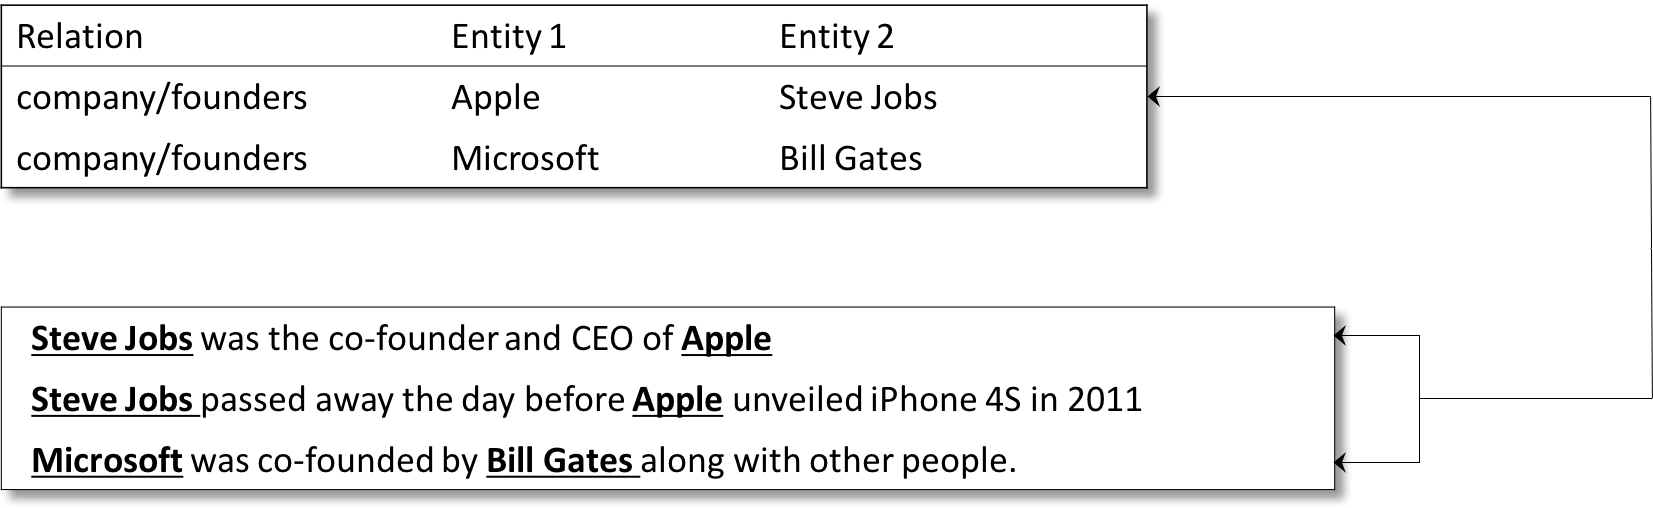
\includegraphics[width=0.85\linewidth]{Images/Relation-Example.png}
    \caption{A depiction of relation extraction task showing positive and negative examples along with the annotated entities in the source text}
    \label{figure:relation-extraction-example}
\end{figure}
    
\section{The GWAS catalog}
\label{section:gwas-catalog}
A genome-wide association study (GWAS) is an approach to detect genetic variations associated with particular disease or traits by scanning markers across the genomes of a large-scale sample of subjects in a high throughput manner. In less than a decade, GWAS studies have successfully produced discovery of new genetic associations which have led to the development of new strategies to diagnose, treat and prevent diseases. This increase in GWAS research calls for a database that allows researchers to query and search for previous results quickly. Such a database has been created and maintained online by the National Human Genome Research Institute (NHGRI)\footnote{\textbf{NHGRI}: \url{https://www.genome.gov/}} called A Catalog of Published Genome-Wide Association Studies (Catalog of GWAS) \cite{hindorff2011catalog}. This database provides a resource to overview scientific investigations, summarization of associated genetic sites and may help suggest genes that are responsible for phenotypic traits in humans. 

The Catalog of GWAS was first released on November 25, 2008, with more than 5,000 entries available for search \cite{welter2014nhgri}. Since then, a large number of new GWAS articles have been published, and the catalog is regularly updated by systematically selecting research articles reporting large-scale GWAS. NHGRI continues to update and curate the catalog regularly by a team of expert curators who manually select study-level fields of information from published GWAS and add them to the catalog. As of September 21, 2016, the Catalog of GWAS contains approximately 29,000 entries extracted from nearly 2,200 discrete articles covering more than 1500 diseases and traits. 

Figure \ref{figure:gwas-catalog-example} shows an example entry in the Catalog of GWAS. Each entry represents an observed association reported in an article, specifying that an association between the genetic variant and a phenotype was observed from this study from an initial stage sample. This information is marked in database as \emph{Strongest SNP}, \emph{disease/ traits} and \emph{Initial Sample Size} fields respectively. The entry also specifies that the observations were validated with a replication sample, given in the \emph{Replication Sample Size} field and the whole study was conducted on a particular group of people, marked in the \emph{Ethnicity} field. These data fields describe the characteristics of the population samples used in the GWAS studies and are the focus of this thesis. Other data fields include the information about where the genetic variant resides in the genome and statistical strength of the observation and hold importance from the biomedical research perspective.  

\begin{figure}[ht]
    \centering
    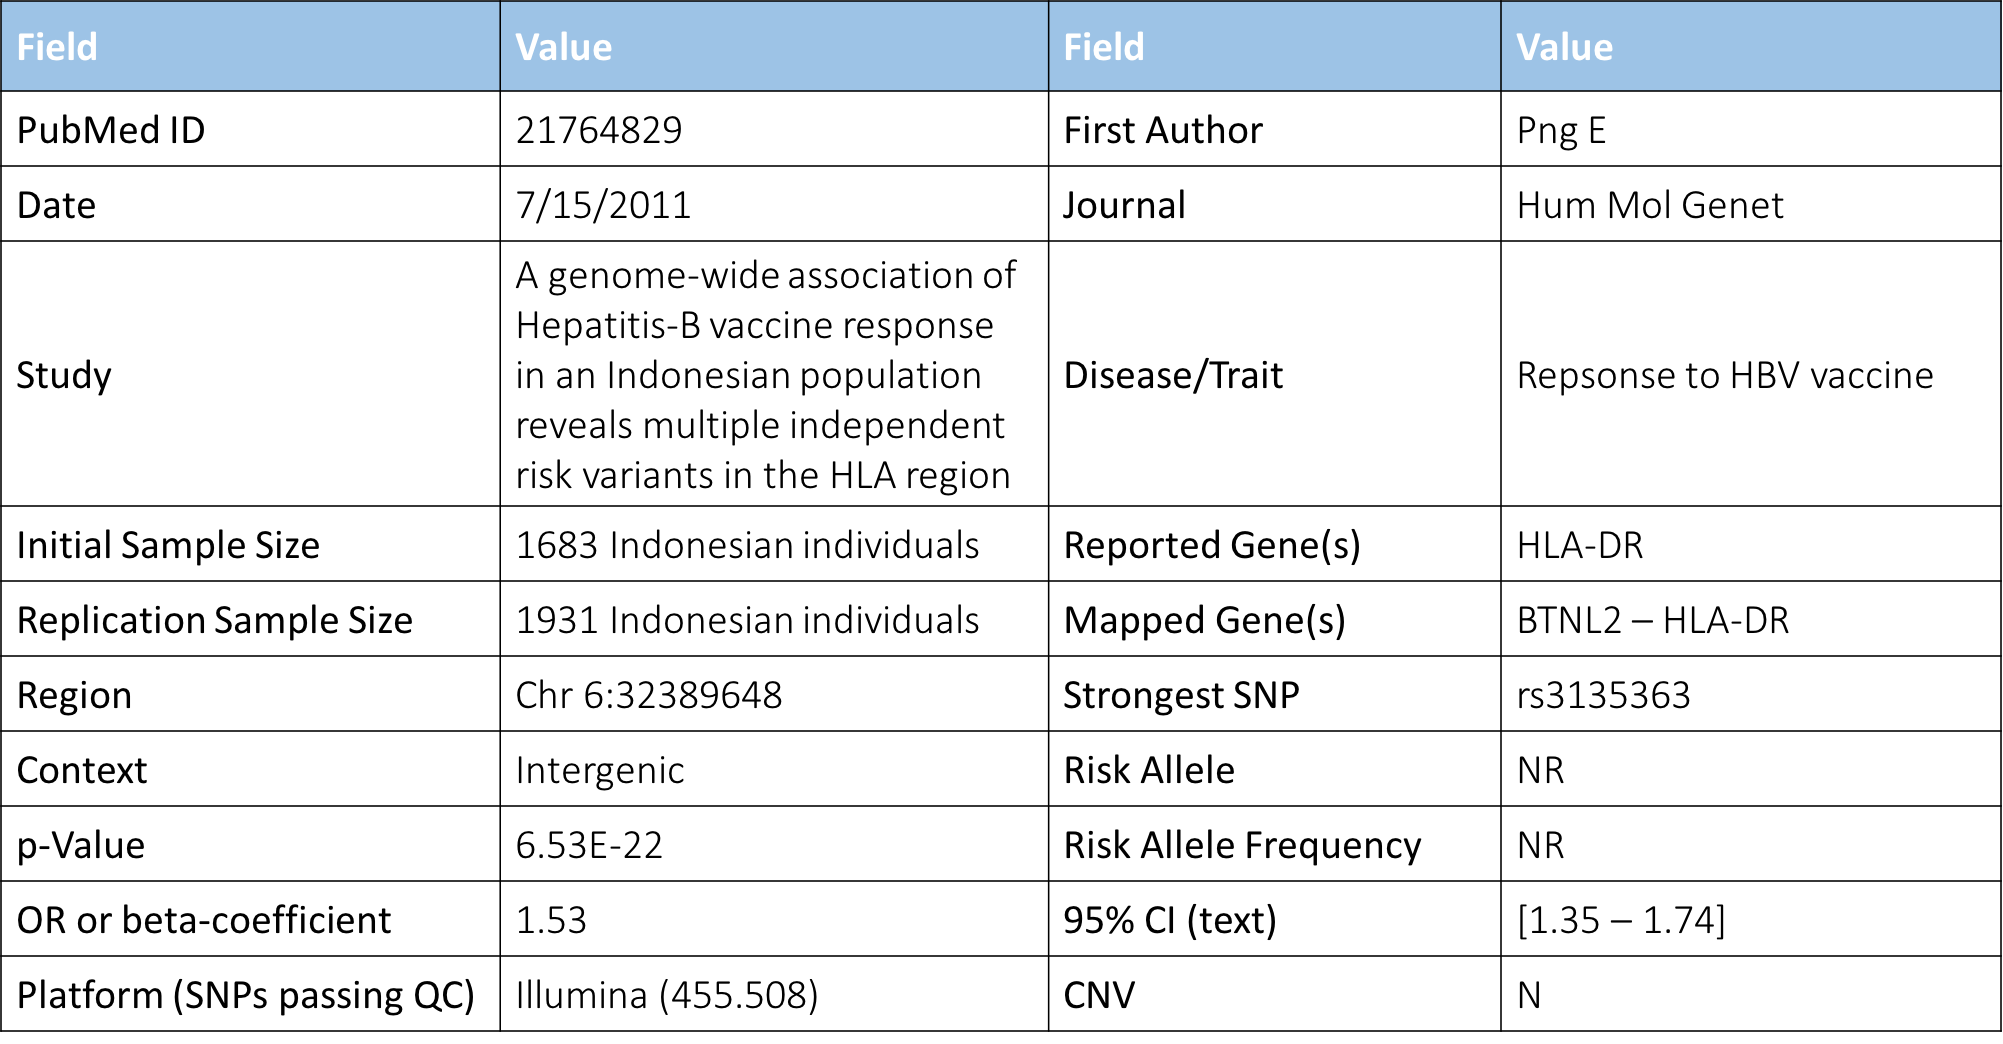
\includegraphics[width=0.85\linewidth]{Images/GWAS-Example.png}
    \caption{Example of an entry in the Catalog of GWAS showing different fields and their corresponding values from a sample text.}
    \label{figure:gwas-catalog-example}
\end{figure}

\section{The Problem}
\label{section:problem}
Our goal is to automate the extraction of the study-level data fields from GWAS articles using a Machine Learning approach to Natural Language Processing. In this thesis, we primarily focus on the characteristics of the sample populations employed in the experiments, i.e. the experimental stage (``\emph{initial}'' or ``\emph{replication}''), the ethnicity groups of the individual involved and the size of the sample population pool. We aim to extract these information fields in the form of tuples {\it <stage, ethnicity>} and {\it <stage, sample size>} and therefore reach the final entries for the database. Collaborative work \cite{jain2016weakly} has been performed for extracting other data fields towards a larger goal of obtaining all the information recorded in the Catalog of GWAS.

This task of automatic extraction of relational information is important as the curation of this knowledge base is primarily done by a team of experts with in-depth domain knowledge which is highly expensive and time-consuming. Various epidemiologists from NHGRI and more recently European Bioinformatics Institute (EBI)\footnote{\textbf{EBI}: \url{http://www.ebi.ac.uk}} manually curate the database on a weekly basis using the information from the published scientific literature. This operation primarily involves the professionals reading articles, extracting key findings and cross-referencing the data all of which can be prone to human errors. Also, as the volume of biological literature grows rapidly, it becomes increasingly difficult for these experts to keep pace with the published data thus creating a pressing need to assist curation with automated tools. 

An example of matched results of the entry in the GWAS catalog with the actual passages in the text of the article is depicted in the Figure \ref{figure:problem-example}. These results can be expressed in the form of previously mentioned tuples which usually exhibit a semantic and/or lexical relationship between its elements. The process of extraction of such relations between the entity pairs from the text plays a vital role in information extraction and subsequent knowledge base population. These relation extraction tasks are based on text mining and information extraction which are derived from various machine learning and natural language processing strategies.

\begin{figure}[ht]
    \centering
    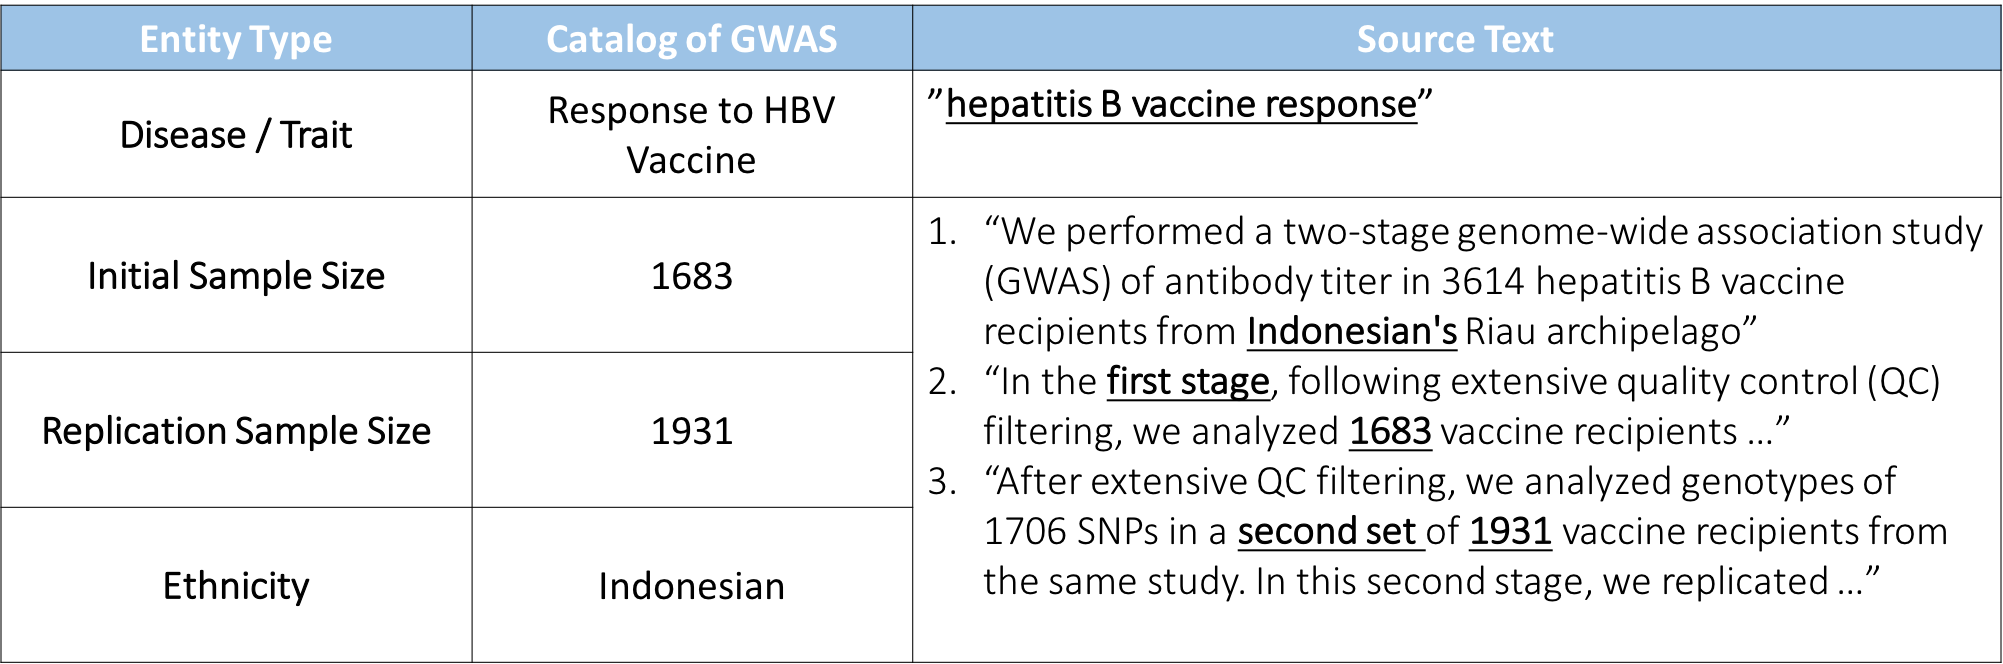
\includegraphics[width=0.85\linewidth]{Images/Problem-Example.png}
    \caption{Example of the curated data in the Catalog of GWAS entry matched to different passages in the text from source article}
    \label{figure:problem-example}
    \vspace{0.2in}
\end{figure}

\section{Our Approach}
\label{section:our-approach}
This thesis presents and implements a general approach to extraction of entity pairs which exhibit a given relationship from biomedical databases. The key idea is to use machine learning and natural language processing to understand the underlying structure of these relations using existing literature and extract the entity pairs from new content which adhere to this composition. Most existing methods leverage various tools of linguistic analysis like parsing, chunking, etc. to transform the relation mentions into some rich representation which can be used by some statistical classifier such as Support Vector Machines (SVM) \cite{hong2005relation} or Maximum Entropy (MaxEnt) \cite{yao2010multi}. Features used by such natural language processing tools are often hand-designed and are subjected to error propagation introduced by their imperfect quality. 

This thesis targets an independent relation extraction system that both avoids complex feature engineering and minimizes the reliance on NLP modules, potentially alleviating error propagation and advancing our performance. We employ convolution neural networks (CNNs) that can extract $n$-grams from the raw sentences and induce an abstract representation which is capable of capturing underlying semantic and syntactic properties of words. Our method uses the tokenized words as input without any complicated pre-processing which are subsequently transformed into vectors by looking up word embeddings. These vectors are used to extract lexical and semantic features using a convolutional approach in the form of various feature maps. These maps are then used to create a final feature vector which is fed to a logistic regression function for final output. This approach to natural language processing using convolution neural networks has been intensively studied but, to the best of our knowledge, never been applied to the problem of learning from curated data and knowledge base population.

We implement the approach as mentioned above and apply it to two problems of relation extraction from the biomedical literature. The first task is to extract pairs of stage (initial or replication) and ethnicity background of the study samples from the GWAS articles and the second task is to obtain pairs of the ethnicity and sample size from the same GWAS studies. Both these tasks use the already curated data from the Catalog of GWAS as the training examples. The existing curated data from the GWAS catalog is matched to text to create the training examples for our neural networks. However, as this matching is not trivial and involves various natural language processing tools, we will discuss it briefly in the subsequent chapters. Collaborative work, out of scope for this thesis, is also done on the task of annotating scientific literature using various crowd-sourcing techniques. 

This approach of relation extraction is not limited to use for the GWAS Catalog. A huge number of different biomedical databases are available today, and many are similar to GWAS such that they contain data derived either through manual curation by teams of experts or structured information submitted by authors or researchers directly from published literature. Apart from the biomedical domain, this approach is equally applicable to other areas which can benefit from the extraction of structured information from freely available text. We intend our approach to be generalizable across these databases and to other relation extraction problems as well. 

\section{Related Work}
\label{section:related-work}
Relation extraction is one of the most widely studied topics in Natural Language Processing. The task of relation extraction is to understand the relationship between a pair of entities from the text and predict new pairs exhibiting same association from other textual sources. There is considerable interest in automatic relation classification, both as an end in itself and as an intermediate step in a variety of natural language processing applications. 
Research in the field of relation extraction dates back as far as the late 1970s. In 1975, Riesbeck and Schank \cite{riesbeck1976comprehension} published work on ELI, an English Language Interpreter, which was able to produce structured representations of the semantic information in stories. In the mid-1980s, Andersen et. al. \cite {andersen1992automatic} launched a commercial data extraction product known as JASPER (Journalist's Assistant for Preparing Earnings Reports) which provided real-time financial news to traders. From 1987 until 1988, a series of competition-based conferences known as Message Understanding Conferences \cite{grishman1996message} led to the refinement of ideas, methods and evaluation strategies related to information extraction and natural language processing. In an effort to improve the performance of automated relation extraction systems, there was a fundamental shift in using various machine learning approaches for such tasks. With more development in the fields of statistics, machine learning, and natural language processing, researchers started applying different machine learning paradigms to the task of natural language processing.  

\subsection{Supervised Learning}
\label{subsection:supervised-learning}
Various supervised systems for relation extraction have been studied extensively since rich annotated linguistic resources have been released. In these supervised approaches, sentences (or part of sentences) in a corpus are either hand-labeled or heuristically annotated for the presence of entities which exhibit a relationship between themselves. A supervised relation extraction system has three steps: 1) data representation for labeled examples e.g. feature extraction for feature-based methods or extracting objects for kernel-based methods 2) train a classification model as the relation detector/classifier 3) apply the model as the relation extractor on the unseen relation mentions. 

One of the most studied relation extraction tasks is the Automatic Content Extraction (ACE)\footnote{\textbf{ACE}: \url{http://www.itl.nist.gov/iad/mig/tests/ace}} relation extraction evaluation sponsored by the U.S. government. In general objective, the ACE program is motivated by and addresses the same issues as the MUC program that preceded it and was convened by the NIST\footnote{\textbf{NIST}: \url{http://www.nist.gov}} from 1999 to 2008. ACE 2005 defined seven major entity types such as PER (Person), LOC (Location), ORG (Organization) and also identifies seven major relation types and more than 20 subtypes. ACE provides a large corpus which is manually annotated with entities, relations, events, and values. In this task, each relation mention expressing one of the predefined types is tagged with a pair of entity mentions appearing in the same sentence as its arguments. More details on ACE evaluation can be found on the official ACE website. 

For data representation, state-of-the-art methods are either feature-based or kernel-based. Given a relation mention, a feature-based method extracts a rich list of structural, lexical, syntactic and semantic features and convert these extraction clues into feature vectors \cite{guodong2005exploring} \cite{nguyen2014employing}. In contrast, kernel-based methods represent each instance with an object such as augmented token sequences or a parse tree and use a carefully designed kernel to calculate their similarity \cite{qian2008exploiting} \cite{culotta2004dependency}. These approaches for data representation are practical because they leverage a large body of linguistic knowledge resources. 

Different machine learning methods have been applied for relation extraction tasks. The two most popular ones are maximum entropy classifiers (MaxEnt) \cite{yao2010multi} and support vector machines (SVM) \cite{hong2005relation}. Other methods such as K-nearest neighbors algorithm \cite{grishman2005nyu} and Voted Perceptron learning algorithm \cite{zelenko2003kernel} have also been utilized for this task of relation extraction. One major issue associated with these methods is the production of labeled training data which is expensive and in limited quantity. Also, as these relationships are labeled on a particular corpus, the resulting classifiers tend to be biased toward the corresponding text domain. 

\subsection{Distant Supervision}
\label{subsection:distant-supervision}
Distant supervision was first proposed by Craven and Kumlein \cite{craven1999constructing} where they generate weakly labeled examples by aligning facts in the Yeast Protein Database into the articles that may establish the facts for training an extractor. This paradigm attempts to create training data automatically by leveraging large knowledge bases of facts and corpus. Since then, it has gained popularity in different domains. Bunescu and Mooney \cite{bunescu2007learning} treat each automatically-labeled relation mention as a labeled example and trains an extractor with supervised learning that tolerates incorrect labels of positive examples. 

To provide a more accurate treatment of label noise while capturing the pair-level constraints, Riedel et. al. \cite{riedel2010modeling} proposes to use the Multiple-Instance Learning, which assumes that only at-least-one of the mentions for each tuple entity listed as having a relation in the knowledge base, indeed has the target relation. Multi-Instance Multi-Label (MIML) learning \cite{surdeanu2012multi} further improve it to allow a tuple of entities to have multiple relations. Further, Takamatsu et. al. \cite{takamatsu2012reducing} viewed the problem differently and proposed a method that estimated the probability of each pattern showing each relation, based on automatically labeled dataset. Their algorithm, however, either removes low-probability false positive matches or corrects high-probability false negative matches by filtering such mentions with their corresponding patterns. 

Labeling noise can be reduced by using a more restricted labeling heuristic. For example, Wang et. al. \cite{wang2011relation} assume that only the first sentence in Wikipedia that contains a pair of related entities is a valid relation mention of the corresponding type. KYLIN \cite{wu2007autonomously} proposes three heuristics for labeling Wikipedia text with the infobox. Such heuristics are domain-specific and are not applicable in a more distant yet typical labeling scenario: align Freebase \footnote{Freebase: \url{https://developers.google.com/freebase/}} to newswires. 

Wang et. al. \cite{wang2011relation} uses distant supervision to improve supervised relation extraction. Their method starts with constructing relationship topics from the set of heuristically labeled examples (by distant supervision) using Diffusion Wavelets. They propose SVM kernel that encodes the background knowledge (a set of related topics) as a source for measuring the similarity between relation mentions. The resulting extraction algorithm improves on existing solutions in the Automatic Content Extraction (ACE) relation evaluation dataset.

Notwithstanding this progress in distant supervision, current performance is still quite modest and not satisfactory for practical use. For example, the system very recently described in Multi-Instance Multiple Label \cite{surdeanu2012multi} learning achieves only a recall of 26.9 and a precision of 29.7 on a standard test set. The resulting instances from using distant supervision often suffer from low precision and semantic drifts and are suitable only for some domains.

\subsection{Unsupervised Learning}
\label{subsection:unsupervised-learning}
Unsupervised relation extraction algorithms collect pairs of co-occurring entities as relation instances, extract features for these instances and then apply different clustering techniques to find the major relations in a corpus. These algorithms obtain a string of words between the entities in large amounts of text and clusters and simplify these word strings to produce relation-strings and rely upon tagging in advance, a predefined set of entity types, such as Person, Organization, and Location. The distributional hypothesis theory \cite{harris1954distributional} reflects that the pair of entities that occur in related contexts tend to have similar relations which form the basis for various unsupervised relation extraction algorithms.  

Among different such algorithms, Yoa et. al. \cite{yao2011structured} propose several generative models, broadly similar to Latent Dirichlet Allocation (LDA) for the task of relation extraction. One of their models learns fine-grained semantic classes as relation arguments, but they share the similar requirement of tagging coarse-grained argument types. Most of the unsupervised algorithms for relation extraction uses a quadratic clustering algorithm such as Hierarchical Clustering \cite{hasegawa2004discovering} or K-Means \cite{chen2005unsupervised}. Hasegawa et. al. \cite{hasegawa2004discovering} adopted a hierarchical clustering method to cluster the context of entities and simply select the most frequent words int the contexts to represent the relation between those objects. Similarly, Chen et. al. \cite{chen2005unsupervised} proposed a novel unsupervised method based on model order selection and discriminative label identification to address this problem

With the growth of digital information, the target domain is shifting towards the Web and new methods are being proposed without requiring predefined entity types. Kok and Domingos \cite{kok2008extracting} propose Semantic Network Extractor (SNE) to extract concepts and relations. Based on the second-order Markov logic, SNE uses a bottom-up agglomerative clustering algorithm to cluster relation phrases and argument entities jointly. However, this method requires each entity and relation expression to belong to exactly one cluster and are unable to handle polysemous relations phrases.  

Unsupervised approaches use enormous amounts of data and extract a very large number of relations, and the resulting associations may not be easy to map to the relations needed for a particular knowledge base. 

\section{Layout of Thesis}
\label{section:thesis-layout}
The remainder of this thesis is organized as follows: Chapter 2 describes the data preparation and preprocessing steps required to analyze the input text and use it as an input to the neural networks. Chapter 3 presents the general framework of the convolutional neural network that we are using for our task of relation extraction. Chapters 4 report the implementations of the approach and the results for the two information extraction problems described above along with various extensions to the neural network framework that we employed.  Finally, Chapter 5 summarizes the results, describes the overall conclusions and explores future work.

The material in part from the Introduction is currently being prepared for submission for publication. The thesis author was the primary investigator and author of this material.